%!TEX root = ../PatilM-[RnD-MT]Report.tex

\chapter{State of the Art}
\paragraph{}Over the years, research into qualitative spatial representations has led to the development of various models which can be used to represent the visually observable space.From a more scientific perspective these models are known as ``Qualitative calculi'', the current state of the art calculi rely on a single spatial primitive such as distance, direction, topology etc., to describe a set of relationships amongst the observable objects. In general each calculi comes with its own set of benefits and drawbacks as each one of them has been tailored to exploit different aspects of space\cite{bibid}. 

\paragraph{}For the case of robot navigation, current state of the art approaches utilize qualitative calculi that can provide both spatial and temporal information such as the QTC \cite{bibid} or QRPC \cite{bibid}. There exist comprehensive surveys that provide detailed information about each of the existing qualitative calculi\cite{bibid}, hence this state of the art aims to provide only a concise overview of the qualitative calculi that are advantageous to our application. We shall look into the relationships afforded by each of these calculi and their classification based on the domain of their utility.
 
\section{Forms of qualitative spatial representations}
		%    \item \textcolor{blue}{What have other people done?}
		%    \item The work presented in Alan Blackwell's master thesis \cite{blackwell1988spatial} provides a qualitative method for  representation of two dimensional shape and position and has been used to solve a few simple spatial reasoning tasks, with applications in the field of robotics. While the focus is mainly on the development of a qualitative representation it doesn't particularly focus on the use of this method for robot navigation. The outlined approaches for the use case in robot navigation raises more questions instead of providing a solid practical approach to the problem. 
		
		
		%    \item \cite{chao2014survey}
		%	\item \cite{dondrup2015computational}
		
		\subsection{Topological Representations} \cite{} \cite{bibid} \cite{bibid} : This is the most fundamental spatial representation, wherein the observed space is divided into distinctive regions based either on distinctive points in space or on separable objects found in the space. Topological representations draw heavily from the field of ``Mereology''(the theory of parthood) to describe relations between the distinctive regions. Qualitative calculi such as RCC, Interval Algebra, n-intersections etc. belong to this category. Such representations deal with the ``\textit{invariant properties that are under continuous deformations of objects, including translating, rotating and scaling}'', and often include only spatial information while completely disregarding temporal data. 
		
		\begin{figure}[h]
			\centering
			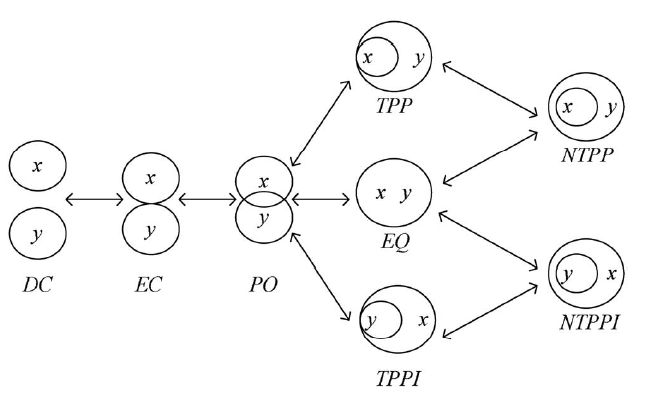
\includegraphics[width=0.7\linewidth]{images/rcc8_rel}
			\caption{The eight jointly exhaustive and pairwise disjoint relations of region connection calculus (RCC8). The arrows show which relation is the next relation a configuration would transit to, assuming the continuous movements or deformations \cite{bibid}, \cite{bibid}, \cite{bibid}.}
			\label{fig:rcc8rel}
		\end{figure}
		
		
		\subsection{Directional Representations} \cite{chen2015survey} : The relative direction between two different objects can be represented using directional relations/representations. These representations rely on three primary elements, a reference object, a reference frame and a target object to define a valid relation between two different objects. Directional representations are widely classified into two categories, point based and projection based with the discerning factor being the dimension of the objects involved and distinction of space using either cone shaped spatial sectors or by using vertical and horizontal lines to create smaller rectangular sectors. Furthermore, the directional calculus isn't restricted to using only cardinal directions, it also allows the use of nominal directional information such as left ,right etc to describe the directional relations. Qualitative calculi such as CDC, OPRA, CyCord etc utilize the directional representation. Being based of topological representations, directional representations also include only spatial information while disregarding temporal data.
		
		\begin{figure}[h!]%
			\centering
			\subfloat[Cone-shaped direction relations \cite{isli1}]{{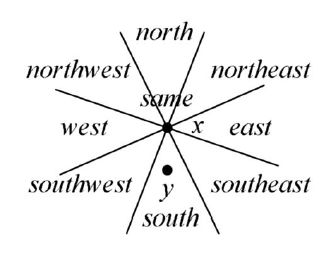
\includegraphics[width=6cm]{images/direction_cone} }}%
			\qquad
			\subfloat[Projection-based direction relations \cite{isli2}]{{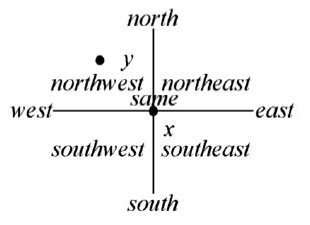
\includegraphics[width=6cm]{images/direction_projection} }}%
			\caption{The point based and projection based direction representations \cite{bibid}}%
			\label{fig:example}%
		\end{figure}
	
		\subsection{Distance Representations} \cite{chen2015survey} : The qualitative representation of spatial distance can be classified into two groups namely absolute and relative. This classification is made solely on the basis of  the presence/absence of an extraneous referential object in the relation between two objects. This distinction can be clearly illustrated by the following example,`the distance between A and B is 8 meters' or `A is near B', this is a absolute approach as the distance is measured directly between two objects.Whereas saying that `A is closer to B than that to C' classifies as a relative approaches as this involves the comparison to a third object.Furthermore, it has been shown that absolute approaches	can be qualitative or quantitative, but relative approaches are commonly qualitative \cite{bibid}.Qualitative calculi such as the ARGD(or Delta) and TPCC use the distance representations to describe the observable space. Distance based relations have found to be insufficient by themselves when it comes to the task of robot manipulation/navigation and hence are often used in combination with distance representations to yield a fairly suitable and complete representation of the environment \cite{bibid}. Like with the direction representations this calculi also lacks temporal data in the encoded relations and is hence unsuitable for applications involving moving objects.
		
		\begin{figure}[h]
			\centering
			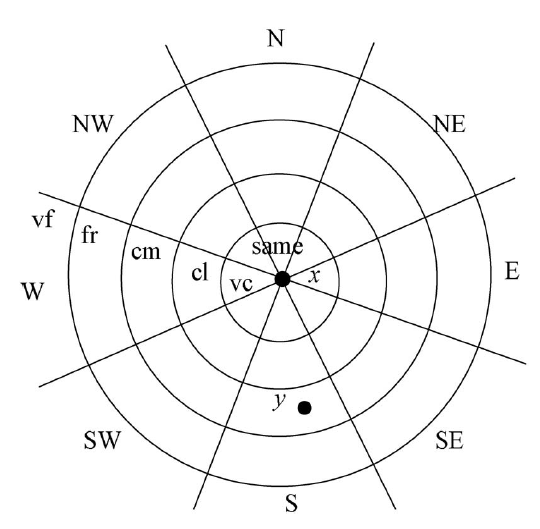
\includegraphics[scale=0.8]{images/argd_delta}
			\caption{An representation of the combination of cone-shaped direction and absolute distance: very
				close(vc), close(cl), commensurate(cm), far(fr) and very far(vf), \cite{bibid}, \cite{clementini1997qualitative}.}
			\label{fig:argddelta}
		\end{figure}
		
		
		\subsection{Moving object Representations} \cite{chen2015survey} : Topological representations, directional representations and distance representations describe relations between stationary objects, this limitation encouraged the development of a moving object representation which can qualitatively represent moving objects and their trajectories. These representations effectively deal with both spatial and temporal data to describe valid relations among mobile objects, while these relations include some directional information they mainly describe the relative motion between two objects and not relative direction. The relative motion between two objects is described using oriented line segments which are approximations of the trajectory of the objects in motion. QTC, QRPC are the two prominent calculi that utilize moving object representations. Moving object representations and the calculi using these representations have been proven to have solved the problem of representing moving objects but since these relations lack any distance information, they are still prone to failure and often need a complimentary distance calculi to ensure that a mobile object(robot) can successfully move around in the given environment without collisions.
		
		\begin{figure}[h]
			\centering
			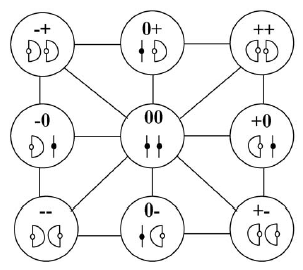
\includegraphics[scale=1]{images/qtcb}
			\caption{Basic relations of basic Qualitative Trajectory Calculus (QTCB) in a conceptual neighborhood diagram. The solid dots represent the stationary objects and the open dots represent the moving objects \cite{bibid}, \cite{de_weghe}.}
			\label{fig:qtcb}
		\end{figure}		
		
		\newpage
		
		\begin{table}[h!]
			\begin{adjustwidth}{-2cm}{}
				\resizebox{\textwidth}{!}{%
					\begin{tabular}{|p{3cm}|p{4cm}|p{3cm}|p{3cm}|p{8cm}|}
						\hline
						\textbf{Domain} & \textbf{Model Name} & \textbf{Type of objects} &\textbf{Number and granularity of relationships} & \textbf{Description} \\ \hline
						\multirow{2}{*}{Temporal} & Interval Algebra \cite{allen1990maintaining} & Time Intervals & 13 relationships, Binary relationships & It does not consider time instants. \\ \cline{2-5} 
						& Extended Interval Algebra  \cite{freksa1992temporal} & Time intervals and extreme points of the intervals & 29 (13 IA(Interval algebra) + 16 extremes), binary & It extends IA(Interval Algebra) model by considering new relationships including the extremes of the interval and it introduces the notion of conceptual neighborhood. \\ \hline
						\multirow{8}{*}{Spatial} & Region Connection Calculus  \cite{randell1992spatial} & Sets & 8 or 5 relationships, Binary Relationships & It uses the geometric properties associated to the connection between two sets to establish relationships that are no longer linear but planar, and which are invariant to translation, rotation and scaling. \\ \cline{2-5} 
						& Cardinal Reference System(CRS)  \cite{frank1992qualitative} & Generic objects & 9 (8 cardinals + 1 neutral) relations, Binary Relationships & It describes the position of any object by using a cardinal orientation as reference system and by adding also a neutral region \\ \cline{2-5} 
						& FFC (Flip Flop Calculus) \cite{ligozat1998reasoning} & Points & 8 (6 + 1 double + 1 triple), Ternary Relations & It is based on the possible positions of a point C with respect to a segment AB defined by other two points, A and B. \\ \cline{2-5} 
						& SCC (Single Cross Calculus) \cite{freksa1992temporal} & Points & 11 (8 +B=C+1 double + 1 triple), Ternary Relations & Describes the possible positions of a point C with respect to a segment AB and the orthogonal line to segment AB on B. \\ \cline{2-5} 
						& DCC (Double Cross Calculus)  \cite{freksa1992utilization} & Points & 17 (15 regions + 1 double + 1 triple), Ternary Relations & Describes the possible positions of a point C with respect to a segment AB and two orthogonal lines to segment AB on A and B. \\ \cline{2-5} 
						& Oriented point based Reasoning  \cite{moratz2006representing}& Oriented Points & 4, Binary Relations & It is based on the relative orientation between pairs of oriented points in terms of two qualitative spatial dichotomies: the front–back and left–right. \\ \cline{2-5} 
						& DRA (Dipole Relation Algebra)  \cite{dylla2004empirical}, \cite{dylla2004exploiting} & Dipoles (or oriented segments) & 24, Binary Relations & It is based on the relative position of oriented segments. \\ \cline{2-5} 
						& OPRA (Oriented Point Relation Algebra)  \cite{dylla2006generalizing} & Oriented points & Depends on the granularity, Binary Relations & As DRA model, it is also based on the relative position two oriented points, but it supports different levels of granularity. \\ \hline
						\multirow{2}{*}{Spatio-temporal} & QTC (Qualitative Trajectory Calculus)  \cite{van2005representing} & Points & 81, Binary Relations & It describes the possible relations among two moving points in terms of the front–back and left–right dichotomies. \\ \cline{2-5} 
						& QRPC (Qualitative Rectilinear Projection Calculus)  \cite{glez2013qrpc} & Oriented points & Depends on the chosen granularity (up to 48), Ternary Relations & It establishes the possible relations of an object with respect to the trajectory of another object depending on the cross-point of the trajectories and the relative position among them \\ \hline
				\end{tabular}}
			\caption{Key features of the more representative models(calculi) of qualitative representations of spatial or temporal domains in the existing literature \cite{glez2013qrpc}.}
			\end{adjustwidth}
		\end{table}
	
			\newpage
	
		\subsection{Conclusion:}From the above breakdown of the representations and the calculi, it is easy to summarize that distance representations and moving object representations are the most promising representations for our application in mobile robot navigation. Consequently the calculi associated with these representations will be the ones that are further scrutinized in the following section. The reasoning behind this conclusion is fairly simple moving object representations are basically spatio-temporal representations which take into account both the spatial and temporal data to create abstractions of the objects trajectory, this is crucial when dealing with mobile objects as this gives a more concrete representation of the objects in motion. In the case of distance representations although these representations deal only with spatial information, they provide explicit information on how close or far the objects under consideration are. Thus effectively capturing the possibility of a collision between the objects, this sort of information cannot be found in the direction and topological representations hence rendering them unfavorable for our application in mobile robot navigation. \cite{art1}
	
	\section{Analyzing qualitative calculi for navigation}
	\paragraph{} This section aims to provide a through understanding at a selective group of qualitative calculi based on the conclusions drawn from the previous section. Namely we shall look at the qualitative calculi such as the QTC, QRPC and ARGD which use moving object representations and distance representations and function in the spatio-temporal and spatial domains respectively.
%	write only theory here
	\subsection{Qualitative Trajectory calculus}
	\paragraph{}\cite{clementini1997qualitative}
	\subsection{Qualitative Rectilinear Projection calculus}
	\paragraph{}
	\subsection{Qualitative Distance calculus}
	\paragraph{}
	

	\section{Implementations of qualitative calculi for navigation}
	
	\begin{itemize}
	\item \cite{chen2006qualitative}, utilizes a teach-relay approach to navigate through indoor and outdoor environments. A sparse optical flow technique is used to extract features in the teach phase and feature matching is done in the replay phase to successfully navigate a given path. The approach uses a qualitative control strategy where motion primitives are obtained by using a voting mechanism in collaboration with the observed features.
	\item \cite{chen2009qualitative},develops a qualitative control algorithm that is able to navigate through both indoor and outdoor environments by using a concept called funnel lane, where the feature coordinates are used to determine turning directions in the replay phase. The algorithm couples odometry information with the funnel lane approach to achieve robust navigation.
	
	\subsection{Implementations}{Examples of implementation of navigation using qualitative control}
	\item \cite{sarcinelli2002using} The research presented in this approach uses optical flow vectors in combination with a confidence measure to control the linear and angular speeds of the robot. Image segmentation is used to split the scene into different objects and a estimation of time of collision for each object is used as a confidence measure for the control commands.
	\item \cite{murali2008autonomous} This approach uses a single monocular gray-scale camera to navigate. The algorithm uses a combination of visual homing and corridor ceiling lights to perform straight-line navigation in an unknown corridor. Although this approach works with both textured and untextured environments it uses a kalman filter(quantitative approach) to achieve localization.

\end{itemize}

\section{....}
Use as many sections as you need in your related work to group content into logical groups

Don't forget to correctly cite your sources \cite{art1}.
\section{Limitations of previous work}

